\begin{frame} [fragile]
\small
	\frametitle{Amplitude and Trigger correlation}
    		\begin{figure}
		 \centering
			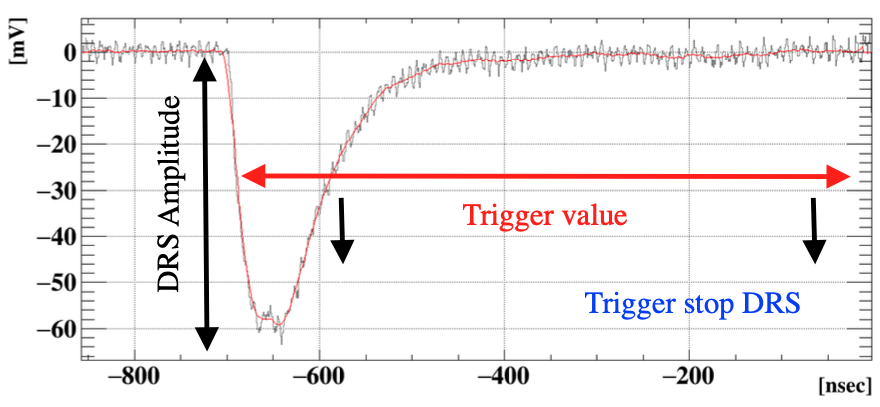
\includegraphics[scale=0.3]{figures/instruments/Waveform_trigger.png}
			\caption{Example Waveform recorded by DRS4}
		\end{figure}  
	\begin{itemize}
		\item By changing the amplitude from a minimum value (300 mV) to a maximum value (full scale), in steps of 25 mV, \colorbox{yellow}{check the linearity} between the amplitude value and the trigger value.
	\end{itemize}
\end{frame}
